%%%%%%%%%%%%%%%%%%%%%%%%%%%%%%%%%%%%%%%%%%%%%%
% Made by:
% Ciudad de Mexico
% Mexico
% Sat Oct 15 10:10:44 UTC 2016
%

\documentclass[a4paper,fleqn,usenatbib,useAMS]{mnras}

\usepackage[T1]{fontenc}
\usepackage{ae,aecompl}
\usepackage{graphicx}	% Including figure files
\usepackage{amsmath}	% Advanced maths commands
\usepackage{amssymb}	% Extra maths symbols
\usepackage[british]{babel}
\usepackage{multicol}        % Multi-column entries in tables
\usepackage{bm}		% Bold maths symbols, including upright Greek
\usepackage{pdflscape}	% Landscape pages


  
\begin{document}

\title{Constraints for two field inflationary models}

%\author[]{    }

% These dates will be filled out by the publisher
%\date{Accepted XXX. Received YYY; in original form ZZZ}
\date{\today}

% Enter the current year, for the copyright statements etc.
%\pubyear{2016}

%\label{firstpage}
%\pagerange{\pageref{firstpage}--%\pageref{lastpage}}
\maketitle


%%%%% ABSTRACT %%%%%%%
\begin{abstract}
XX\\
XX\\
XX\\

\end{abstract}

\begin{keywords}
dark matter  -- galaxy clusters --  gravitation  -- relativity
\end{keywords}



\section{Introduction}
\label{introduction}

XXXXX

XXXXX

XXXXX

XXXXX

XXXXX

\section{Generalities for two field inflationary models}

Although one scalar field models for inflation can be preferable given the fact that they predict only adiabatic like perturbations, two field models can be interesting since there are some regions of parameters were this models can generate small isocurvature perturbations and the addition of new free parameters can help to ''death" single-field inflationary models to bring them back.  

In this section we review in a general way two field inflationary models for inflation following (Ref. Christian T. Byrnes and David Wands). 

\subsection{Background equation of motion}

In this section we consider a two-field inflationary model with canonical kinetic term and where its dynamics is described by an arbitrary interaction potential $V(\phi,\psi)$. As usual we consider that the classical fields are homogeneous and evolve in a FLRW background. Then, the background equation of motion for each scalar field and the Hubble parameter are
\begin{subequations}
\begin{equation}
\ddot{\phi}_i+3H\dot{\phi_i}+V_i=0 \ \ \ (i=\phi,\psi)
\end{equation}
\begin{equation}
H^2=\frac{8\pi G}{3}\left[V+\frac{1}{2}\left(\dot{\phi}+\dot\psi\right)\right],
\end{equation}
\end{subequations}
where $V_i\equiv\partial V/\partial \phi_i$. In the inflationary era it is usually assumed that the scalar fields are slow-rolling. This happens always that the condition $\epsilon_i,|\eta_{ij}|\ll 1$ is fulfill; $\epsilon_i$ and $\eta_{ij}$ are called the slow-roll parameters and are defined in appendix [A]. If this happens we can rewrite the above equations as
\begin{subequations}
\begin{equation}
\dot{\phi}_i\simeq -\frac{V_i}{3H}\left(1+\frac{1}{3}\delta_i^H\right)
\end{equation}
\begin{equation}
H^2\simeq \frac{8\pi G}{3}V\left(1+\frac{1}{3}\epsilon^H\right)
\end{equation}
\end{subequations}
where $\delta^H_i$ and $\epsilon^H$ are new slow-roll parameters defined in appendix [A]. 
\subsection{The adiabatic and isocurvature perturbations}

The equation of motion for the perturbed fields in the spatially flat gauge are (ref)
\begin{equation}
\ddot{\delta\phi}_i+3H\dot{\delta\phi}_i+\sum_j\left[V_{ij}-\frac{8\pi G}{a^3}\frac{d}{dt}\left(\frac{a^3}{H}\dot{\phi}_i \dot\phi_j\right)\right]\delta\phi_j=0
\end{equation}
For the large scales ($k\ll aH$) it is better to work in a rotating basis of the fields given by
  \begin{subequations}
  \begin{equation}
  \binom{\delta \sigma}{\delta s}=S^{\dagger}\binom{\delta \phi}{\delta\psi}
  \end{equation}
  where
  \begin{equation}
  S=\begin{pmatrix}\cos\theta & -\sin\theta\\ \sin\theta & \cos\theta\end{pmatrix}, \ \ \ \tan\theta =\frac{\dot \psi}{\dot \phi}\simeq\pm \sqrt{\frac{\epsilon_\psi}{\epsilon_\phi}}
  \end{equation} 
  \end{subequations}
The field $\sigma$ is parallel to the trajectory and is usually called \textit{adiabatic field} while the field  $s$ is perpendicular to it and is called \textit{entropy field}. 

 If the background trajectory is curved it happens that $\delta\sigma$ and $\delta s$ are correlated at Hubble exit. In this way the power spectrum and cross-correlation at Hubble exit is given by
\begin{subequations}
\begin{equation}
P_{\sigma^*}((k))\simeq\left(\frac{H_*}{2\pi}\right)^2(1+(-2+6C)\epsilon-2C\eta_{\sigma\sigma})
\end{equation}
\begin{equation}
C_{\sigma s^*}(k)\simeq-2C\eta_{\sigma s}\left(\frac{H_*}{2\pi}\right)^2
\end{equation}
\begin{equation}\label{5c}
P_{s^*}(k)\simeq\left(\frac{H_*}{2\pi}\right)^2(1+(-2+2C)\epsilon-2C\eta_{ss})
\end{equation}
\end{subequations}
where $C\simeq 0.7296$ and $\epsilon$ and $\eta_{ij}$ ($i,j=\sigma,s$) are new slow-roll parameters defined in term of the new adiabatic and entropy fields (see appendix [A]).
\subsection{Final power spectrum and spectral index}
The curvature and isocurvature perturbations are defined as
\begin{equation}\label{RS}
R\equiv\frac{H}{\dot\sigma}\delta \sigma, \ \ \ S=\frac{H}{\dot \sigma}\delta s
\end{equation}
In the slow-roll limit in large scales, the evolution of curvature and isocurvature perturbations can be written using the formalism of tranfer matrix (ref) as
\begin{equation}
\binom{R }{S}=\begin{pmatrix}1 & T_{RS}\\ 0& T_{SS}\end{pmatrix}\binom{R}{S}_*
\end{equation}
where
\begin{subequations}
\begin{equation}
T_{SS}(t^*,t)=\exp\left(\int^t_{t^*}\beta Hdt'\right), \ \ \
\end{equation}
\begin{equation}\label{TRS}
T_{RS}(t^*,t)=\exp\left(\int^t_{t^*}\alpha T_{SS}Hdt'\right)
\end{equation}
\end{subequations}
and at linear order in slow-roll parameters
\begin{equation}
\alpha\simeq -2\eta_{\sigma s}, \ \ \ \ \beta\simeq-2\epsilon+\eta_{\sigma\sigma}-\eta_{ss}
\end{equation}

In the other side the primordial curvature perturbation, during radiaton-dominates era some time after inflation has ended, is given in large scales by
\begin{equation}
R=\Psi+\frac{H\delta\rho}{\rho}
\end{equation}
where $\Psi$ is the gravitational potential. The conventional definition of the isocurvature perturbation for an $i$ specie is given relative to the radiation density by
\begin{equation}
S_i=H\left(\frac{\delta\rho_{i}}{\rho_{i}}-\frac{\delta\rho_\gamma}{\rho_\gamma}\right).
\end{equation}
Then, the final power spectrum at the beginning of the radiation-domination era is given by
\begin{subequations}\label{spectrums}
\begin{equation}\label{PRf}
P_R\simeq P|_*(1+\cot^2\Delta),
\end{equation}
\begin{equation}
P_S=T^2_{SS}P|_*,
\end{equation}
\begin{equation}
C_{RS}=T_{RS}T_{SS}P_R|_*
\end{equation}
\end{subequations}
where at linear order in slow-roll parameters
\begin{equation}
P|_*=\frac{1}{2\epsilon}\left(\frac{H_*}{2\pi M_{pl}}\right)^2
\end{equation}
with $M_{pl}$ the Planck mass and $\Delta$ is the observable correlation angle defined at lower order as
\begin{equation}
\cos\Delta =\frac{T_{RS}}{\sqrt{1+T_{RS}^2}}.
\end{equation}
The final scalar tilts, defined as $n_x=d\ln P_x/d\ln k$, at linear order in slow-roll parameters are
\begin{subequations}\label{tilts}
\begin{eqnarray}
n_R&\simeq & -(6-4\cos^2\Delta)\epsilon+2\sin^2\Delta\eta_{\sigma\sigma}\nonumber \\ &&+4\sin\Delta\cos\Delta\eta_{\sigma s}+2\cos^2\Delta\eta_{ss}\\
n_c&\simeq &-2\epsilon+2\tan\Delta\eta_{\sigma s}+2\eta_{ss}\\
n_S&\simeq & -2\epsilon+2\eta_{ss}
\end{eqnarray}
\end{subequations}

In order to understand what is the contribution of our dark matter candidate to the primordial spectrum, it is better to rewritte the primordial adiabatic and entropy perturbations on super-horizon scales as a power law, given by
\begin{subequations}\label{PswAs}
\begin{equation}\label{PrAs}
P_R=A_r^2\left(\frac{k}{k_0}\right)^{n_{ad1}}+A_s^2\left(\frac{k}{k_0}\right)^{n_{ad2}}
\end{equation}
\begin{equation}\label{PrCrs}
C_{RS}=A_SB\left(\frac{k}{k_0}\right)^{n_{cor}}
\end{equation}
\begin{equation}\label{PsAs}
P_s=B^2\left(\frac{k}{k_0}\right)^{n_{iso}}
\end{equation}
\end{subequations}
where at linear order $n_{ad1}=-6\epsilon+2\eta_{\sigma\sigma}$, $n_{ad2}=2n_C-n_S$, $n_{cor}=n_c$, $n_{iso}=n_S$. We have that $A_r^2$, $A_s^2$ and $B$ can be written in terms of the correlation angle as
\begin{subequations}
\label{RelAs}
\begin{equation}
A_r^2=[P_R\sin^2\Delta]_{k_0}, \ \ \ \ A_s^2=[P_R\cos^2\Delta]_{k_0},
\end{equation}
\begin{equation}
B^2=[T_{SS}^2 P_R|_*]_{k_0}
\end{equation}
\end{subequations}
$A_r^2$ and $A_s^2$ are the contribution of the adiabatic and entropy fields to the amplitud of the primordial adiabatic spectrum. 
\subsection{Gravitational waves}

Given the fact that scalar and tensor perturbations are decoupled at linear order, the gravitational waves at horizon crossing is the same than in the case of a single field and the amplitude of gravitational waves remains frozen-in on large scales after Hubble exit during inflation. In this way the power spectrum and the tilt of the gravitational waves is given by
\begin{equation}
P_T=P_{T*}\simeq 8 \left(\frac{H_*}{2\pi M_{pl}}\right)^2(1+2(-1+C)\epsilon)
\end{equation}
\begin{equation}\label{tiltsnt}
n_T\simeq -2\epsilon\left[1+\left(\frac{4}{3}+4C\right)\epsilon+\left(\frac{2}{3}+2C\right)\eta_{\sigma\sigma}\right]
\end{equation}

The tensor-to-scalar ratio at Hubble exit is the same than in the single field. However, at super-horizon scales, the curvature perturbations continue evolving as \eqref{PRf}. In this way the tensor-to-scalar ratio some time after the end of inflation is
\begin{equation}
r\simeq 16\epsilon \sin^2\Delta\left[1-\left(\frac{4}{3}+4C\right)\epsilon +\left(\frac{2}{3}+2C\right)\eta_{\sigma\sigma}\right]
\end{equation}
\section{Experimental constraints for inflationary parameters}

\textcolor{red}{Meter aqu\'i las constricciones experimentales que hay con Planck.}

%
%
%
%
%
%
\section{Simplest scenario: The one field straight scenario and constraints for SFDM models}

The simplest scenario is to consider that only one scalar field was dynamically important during inflation and the extra scalar field observer contributed to the primordial spectrum by generating only isocurvature fluctuations. Even tough the idea of adding an extra spectator that does not contribute for inflation could be considered as no necessary, there are at least two scenarios where this extra degrees of freedom can be important. First is the so called curvaton inflationary model (ref), where it is consider that this new field is responsible for the majority of the adiabatic perturbations. This scenario has been well studied in the literature (ref) and now a days it is one of the preferable scenarios for inflation (ref). In the other side we can consider an scenario where this extra scalar field can be used as a Dark Matter candidate, in such case we will have isocurvature constraints for our model. 

\subsection{Curvaton scenario}

\subsection{SFDM spectator scenario}
The idea of scalar fields as the DM of the Universe was first suggested in (Baldeshti et al. (1983)) and rediscovery by various authors with different names (see e.g. Membrado et al. 1989; Press et al. 1990; Sin 1994; Ji $\&$ Sin 1994; Lee $\&$ Koh 1996; Sahni $\&$ Wang 2000; Peebles 2000; Goodman 2000; Matos $\&$ Ure\~na-L\'opez 2000; Matos $\&$ Arturo Ure\~na-L\'opez 2001; Wetterich 2001; Arbey et al 2001; Woo $\&$ Chiueh 2009; Lundgren et al. 2010; Calabrese $\&$ Spergel 2016; Schwabe et al. 2016; Hui et al. 2017; Moez et al. 2017, among others), for example: SFDM (Matos $\&$ Guzm\'an 2000), fuzzy DM (HU et al. 2000), wave DM (Bray 2010; Schive et al. 2014a), Bose-Einstein condensate DM (B\"omer $\&$ Harko 2007) or ultra-light axion DM (Marsh $\&$ Ferreira 2010). \textcolor{red}{(Completar este p\'arrafo diciendo que el modelo es un candidato serio y meter m\'as referencias).} 


In this scenario we need that the SFDM candidate being a stable spectator field and that its classical dynamics during inflation being negligible. We can obtain such scenario by considering that the trajectory in the field space evolves in the inflaton direction $\phi$ whereas the direction perpendicular to the trajectory corresponds with the SFDM $\psi$. Notice that it is necessary to have $\eta_{\sigma s}=\eta_{\psi\phi}=0$ and that our dark matter candidate evolves much slower than the inflaton. Then, we can see that the last conditions demand that the potential can be written as $V(\phi,\psi)=V(\phi)+V(\psi)$ and $\epsilon_\psi\ll \epsilon_\phi$.

During the inflationary scenario the entropy and adiabatic perturbations are uncorrelated which implies that $T_{RS}=0$ (and $C_{RS}=0$) as can be seen from \eqref{TRS} imposing initial conditions at horizon crossing. In this way we have that $\cos\Delta =0$. 

As is expected from \eqref{PrAs} and \eqref{RelAs} in the inflationary scenario the primordial power spectrum for the adiabatic perturbations is produced purely by the inflaton while quantum fluctuations of the scalar field dark matter give entry to the generation of uncorrelated isocurvature perturbations. In this way the primordial power spectrum of adiabatic, isocurvature and tensor perturbations are
\begin{subequations}
\begin{equation}
P_R=P_R|_*
\end{equation}
\begin{equation}\label{PS1}
P_s=T_{SS}^2 P_R|_*
\end{equation}
\begin{equation}
P_T=\frac{8}{M_{pl}^2}\left(\frac{H_*}{2\pi}\right)^2
\end{equation}
\end{subequations}
and from \eqref{tilts} and \eqref{tiltsnt} the tilts at linear order are
\begin{subequations}
\begin{equation}
n_R\simeq-6\epsilon+2\eta_{\phi\phi}
\end{equation}
\begin{equation}
n_s\simeq-2\epsilon+2\eta_{\psi\psi}
\end{equation}
\begin{equation}
n_T\simeq -2\epsilon
\end{equation}
\end{subequations}
Finally the tensor-to-scalar ratio in this scenario is the same than in the single-inflaton scenario
\begin{equation}
r\simeq 16\epsilon
\end{equation}
which implies that the SFDM observer does not contribute to $r$.

The adiabatic scalar amplitude of perturbations generated during inflation is (ref) 
$A_r^2=2.19\times 10^{-9}
$ which implies that the perturbations for the scalar field dark matter in this scenario is given by $B^2=2.19\times 10^{-9}T_{SS}^2$ where $T_{ss}^2$ depends of the model of inflation that we are considering. It happens that in exactly de-sitter inflation $\epsilon\sim 0$ we have $T_{SS}^2=1$. 

\subsubsection{Initial condition from inflation and constraining isocurvature perturbations}

In this scenario and considering that the dark matter is only composed of SFDM, the perturbation evolution for photons, neutrinos, barions and dark matter start from the initial conditions $\frac{3}{4}\delta_{\gamma}=\frac{3}{4}\delta_\nu=\delta_b\simeq 0$ and $\delta_{SFDM}=A_{SFDM}$ where $\delta_{\alpha}=\delta \rho_\alpha/\rho_\alpha$ and $A_{SFDM}$ is the gauge invariant entropy perturbation
\begin{equation}
A_{SFDM}=\delta_{SFDM}-3\frac{\delta T}{T}
\end{equation}
The fact that $\delta_{SFDM}\gg \delta_{\gamma}$ implies that $\delta_{SFDM}\gg 4\delta T/T$ and then $A_{SFDM}=\delta_{SFDM}$. Notice, from \textcolor{red}{(eq)}, that $\rho_{SFDM}\propto |\psi|^2$ and then we can rewrite $\delta_{SFDM}$ as 
$\delta_{SFDM} = 2\delta \psi/\psi_i
$,
where $\psi_i$ is the SFDM background value during inflation. In this way we can obtain a primordial isocurvature perturbation for a SFDM candidate as
\begin{equation}
P_{SFDM}(k)=\left(\frac{H_*}{\pi \psi_i}\right)^2
\end{equation}

Since SFDM behaves similar to LCDM at cosmological levels, the CMB constraints on CDM isocurvature perturbations applies to SFDM as well. By relating the isocurvature power spectrum with the curvature power as
\begin{equation}
P_{SFDM}(k)=\frac{\beta_{iso}(k)}{1-\beta_{iso}(k)}P_R(k)
\end{equation}
we obtain constraints given by Planck (ref) at the pivot scale $k_0/a_0=0.05Mpc^{-1}$ and for uncorrelated and scale-invariant isocurvature perturbations 
\begin{equation}
\beta_{iso}(k_0)<0.038 \ \ \ \ \ (95\%\ \ \text{C.L., TT, TE, EE$+$lowP})
\end{equation}
This last expression can be extrapolated to impose upper constraints to the mass for our SFDM candidate in terms of the upper limit of the tensor to scalar ratio (see (ref))
\begin{equation}
r<2\times 10^{-4}\left(\frac{g_{*osc}}{3.36}\right)^{-3/4}\left(\frac{g_{s*osc}}{3.91}\right)\left(\frac{m}{10^{-22}}\right)^{-1/2}
\end{equation}
where $g_{*osc}$ and $g_{s*osc}$ are the number of degrees of freedom at SFDM and entropy oscilations. Given that our SFDM candidate starts its oscilation at radiation-domination epoch (when its mass $m\sim H$), we can take $g_{*osc}=3.36$. Taking $g_{s*osc}=3.91$ we can obtain a direct constrain for the scalar field mass for inflation as 
\begin{equation}
\frac{m}{10^{-22}\ eV}<\left(\frac{2\times 10^{-4}}{r}\right)^2
\end{equation}

In ref. (ref) it was obtained the above expression thinking in the SFDM candidate as an axion-like particle, it is, a field that is created by a missalignment mechanism. However, we can see that such result can be extrapolated for whichever SFDM candidate as general constraints for it if the scalar field coexist with the inflaton. We can observe in figure \ref{constraintsSFDM} such constraints in the m vs r plane. As we can see if $r$ is detected in the near future, it will ruled-out models where more massive scalar fields could coexist with the inflaton during inflation. This constraints are important given that in (ultra-light axion like DM must be presented during inflation) it was demonstrated that an ultra-light axion-like dark matter candidate must be presented during inflation. Then, if $r$ is detected in the near future, it could represent an strong constraint for the axion-like particle model. Notice that if we relax the scalar field mechanism under this particle is created, we should expect that this restrictions can be less affective to the model if we consider that the SFDM candidate was created after inflation. 

\begin{figure}
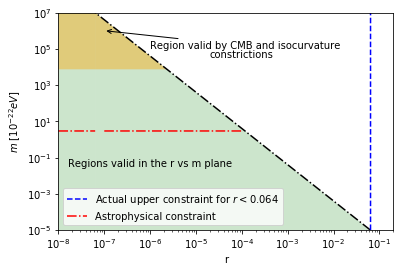
\includegraphics[width=8cm]{SFDMconstraints.png}
\caption{Isocurvature constraints for the SFDM candidate.}\label{constraintsSFDM}
\end{figure}
\section{Constraining two field models with last data}
\section{Conclusions}
\appendix
\section{Slow-Roll index}
\end{document}